\documentclass[a4paper,twoside,11pt]{article}
\usepackage{a4wide,graphicx,fancyhdr,amsmath,amssymb}
\usepackage{algorithmic}

%----------------------- Macros and Definitions --------------------------

\setlength\headheight{20pt}
\addtolength\topmargin{-10pt}
\addtolength\footskip{20pt}

\newcommand{\N}{\mathbb{N}}
\newcommand{\ch}{\mathcal{CH}}
\everymath{\displaystyle}
\newcommand{\solution}[1]{\noindent{\bf Solution to Exercise #1:}}

\fancypagestyle{plain}{%
\fancyhf{}
\fancyhead[LO,RE]{\sffamily\bfseries\large Technische universiteit Eindhoven}
\fancyhead[RO,LE]{\sffamily\bfseries\large 2IV35 Visualization}
\fancyfoot[LO,RE]{\sffamily\bfseries\large department of mathematics and computer science}
\fancyfoot[RO,LE]{\sffamily\bfseries\thepage}
\renewcommand{\headrulewidth}{0pt}
\renewcommand{\footrulewidth}{0pt}
}

\pagestyle{fancy}
\fancyhf{}
\fancyhead[RO,LE]{\sffamily\bfseries\large Technische universiteit Eindhoven}
\fancyhead[LO,RE]{\sffamily\bfseries\large 2IV35 Visualization}
\fancyfoot[LO,RE]{\sffamily\bfseries\large department of mathematics and computer science}
\fancyfoot[RO,LE]{\sffamily\bfseries\thepage}
\renewcommand{\headrulewidth}{1pt}
\renewcommand{\footrulewidth}{0pt}

%-------------------------------- Title ----------------------------------

\title{\vspace{-\baselineskip}\sffamily\bfseries 2IV35 Visualization Set 3}
\author{Jeroen van Oorschot \qquad Student number: 0721913 \\{\tt j.v.oorschot@student.tue.nl}}

\date{\today}

%--------------------------------- Text ----------------------------------

\begin{document}
\maketitle

\pagebreak
\tableofcontents
\newpage
\section{Dataset}
Because I like to a good glass of wine I took the wine dataset to try and find out what makes a wine taste better or worse. The dataset has some measurements of the wine combined with a quality mark determined by a group of experts. There were 2 sets, one with data about red wine, the other about white wine. While looking at the datasets a few things became clear:

\begin{description}
\item[Quality] \hfill \\ The quality is given in an integer number between 0 (very bad) and 10 (very excellent), this means there is not a lot diversity in it.
\item[Dependencies] \hfill \\ Not all of the data is totaly independent, one very clear example are the columns free sulfur dioxide and total sulfur dioxide where the free sulfur dioxide clearly is a part of the total sulfur dioxide.
\item[Red vs white] \hfill \\ In the red wine dataset there is a total of 1599 wines, while in the dataset for white wines there is a total of 4898 wines.
\end{description}

\section{Applications}
In My application I added a column to the data set named "sulfur dioxide" giving the ratio between  the free sulfur dioxide and the total sulfur dioxide. 
\subsection{Scatter plot}
The first idea that comes to mind when I need to find some correlation between variables is a scatter plot. In this case I wanted to find to find some correlation between one of the variables and the quality. The scatter plot gave examples like shown in figure \ref{SP}. As one can see there is not really a trend visible, and because there is so much data (in this case a sample size of 1599) with so little diversity (only 6 different values on the x-axis) it is not really a good picture to get information from. It is nearly impossible to see a trend in this data so this plot helps nearly nothing.
\begin{figure}[!h]
  \centering
  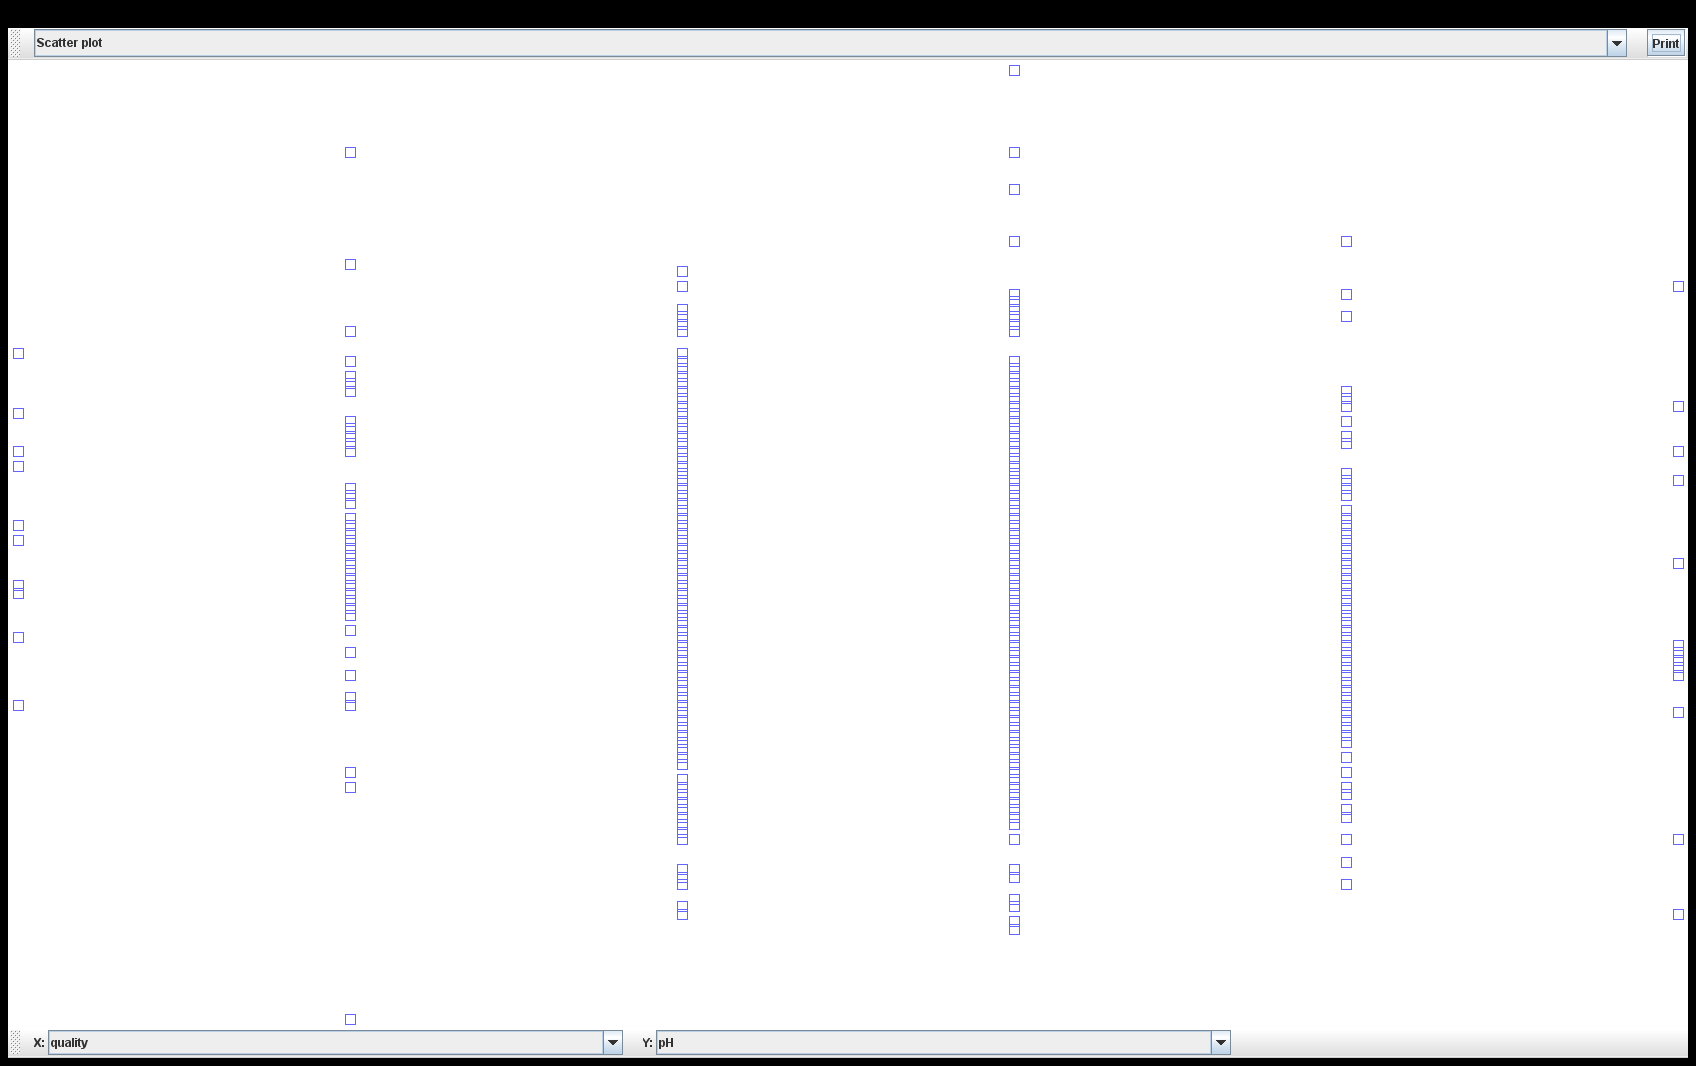
\includegraphics[width=\textwidth]{20131105023902plot.png}
  \caption{Scatter plot of the red wine dataset with quality on the x-axis and pH on the y-axis.}
  \label{SP}
\end{figure}

\subsection{Interval tree}
Since the data set has only so little variations on the quality I came up with a tree structure. I made one root and gave it the columns (except quality) as children. Then every of those children have one child per existing quality. Then every quality has a in advance specified number of children. Those children represent equally sized parts of the total interval. The color indicates which interval we are talking about, the lowest interval is red, the highest is green, the rest is colored according to a continues map from red to yellow and from yellow to green. The size represents what part of the data with that quality lays in the interval. Note that I compute the interval according to the total data set, so it could be possible that a particular quality has a child of size 0 because there simply is no whine in that interval. To allow the user to compare what he likes I made a drag and drop graph with some forces in it to make it better visible, this allows the user to cluster things he want to compare. I also labeled the nodes for more precise information. Because squares are the easiest to compare I used squares as shape, I scaled them in both directions linearly, so we need to compare the sides of the squares, not the area, this is more easy when you hold them next to each other.

\subsection{Median tree}
As I will show in the observations sometimes the Interval tree gave bad results, take for example the case where there is one measurement 10 times bigger that the rest, if we then use 3 intervals we have that measurement alone, an empty interval and the rest in the lowest interval. The tree of such a data set will have only red leaves of size (nearly) 100\% and one green leave, this is obvious not very clear. To resolve this problem I made something quite similar, but now every quality only has 2 children, one for the data bigger that the median, and one for the smaller data.

\section{Observations}
When we start the Interval Tree for White wine we see something like in figure \ref{oit}. We immediately can see that there is an interesting branch at the top slightly to the left. Because we see some big red and also some big green squares we know there is something interesting.

\begin{figure}[!h]
  \centering
  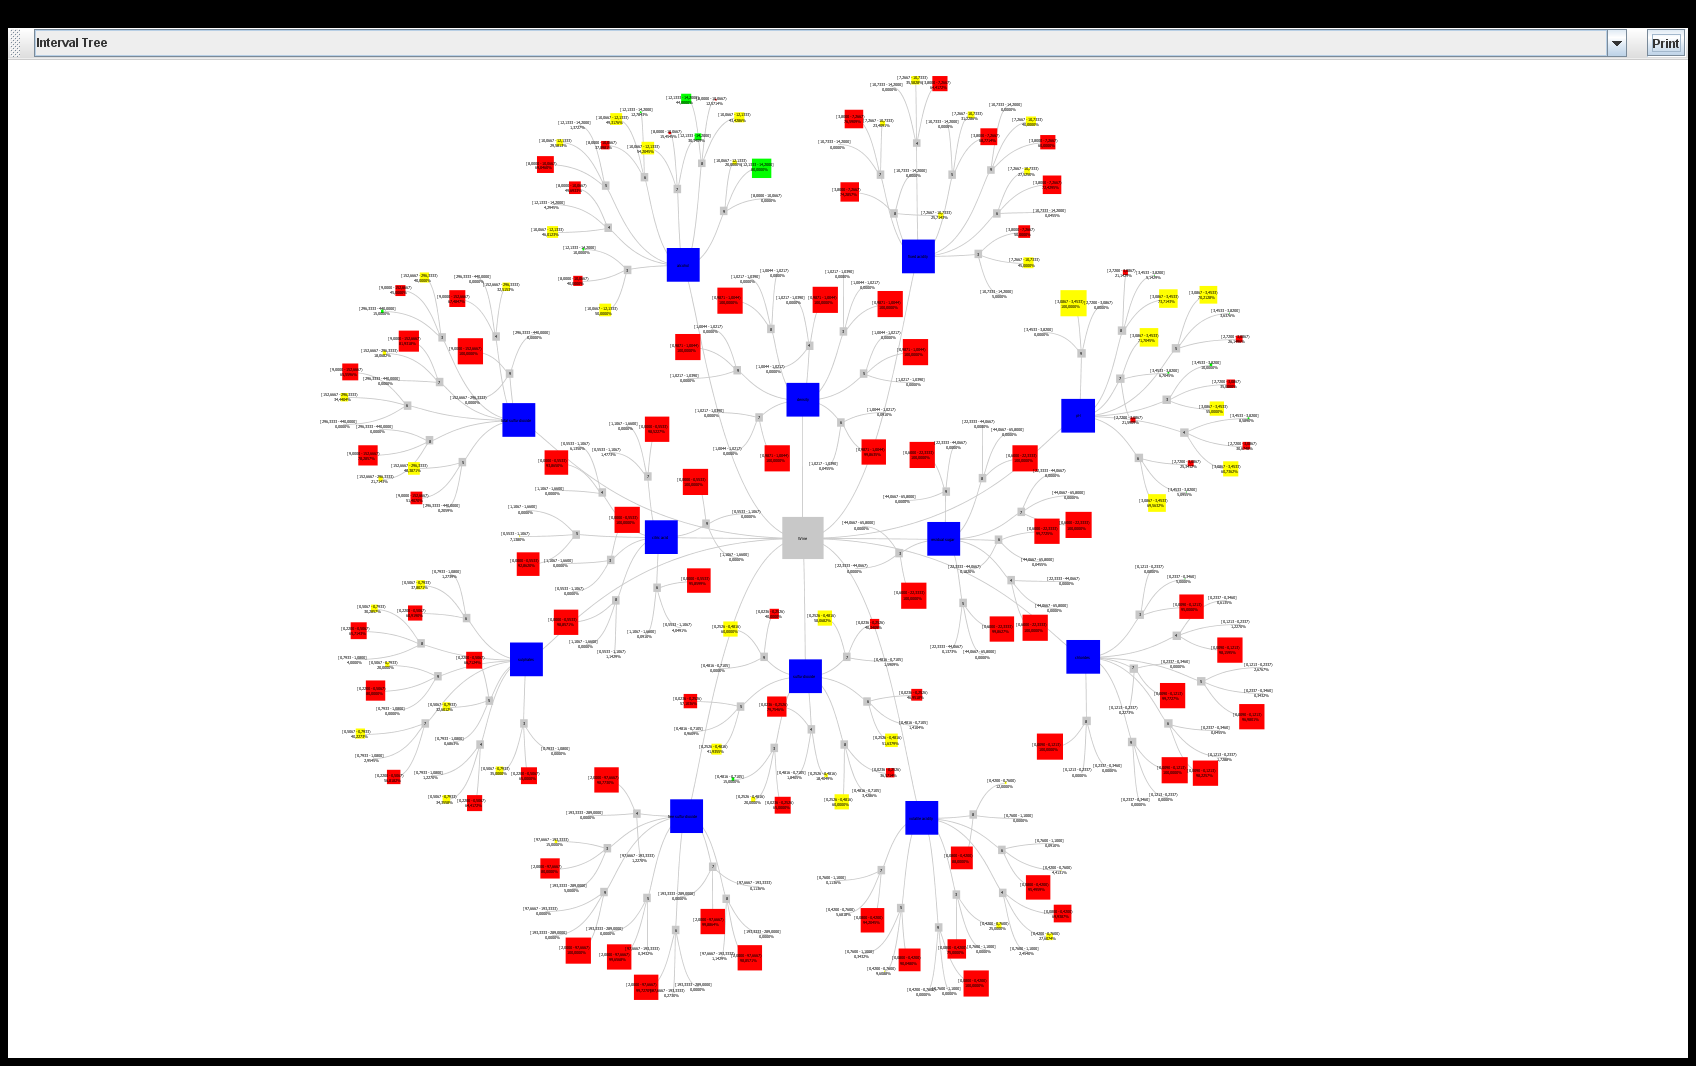
\includegraphics[width=\textwidth]{20131105033557plot.png}
  \caption{Overview with the Interval Tree}
  \label{oit}
\end{figure}

When we zoom in we get a picture like figure \ref{ait}. By looking at the squares we see that the better wines have a relatively bigger green square and a relatively small red square, while for the wines of less quality the opposite holds. From this we can conclude that better wines tend to have a higher percentage of alcohol.
\begin{figure}[!h]
  \centering
  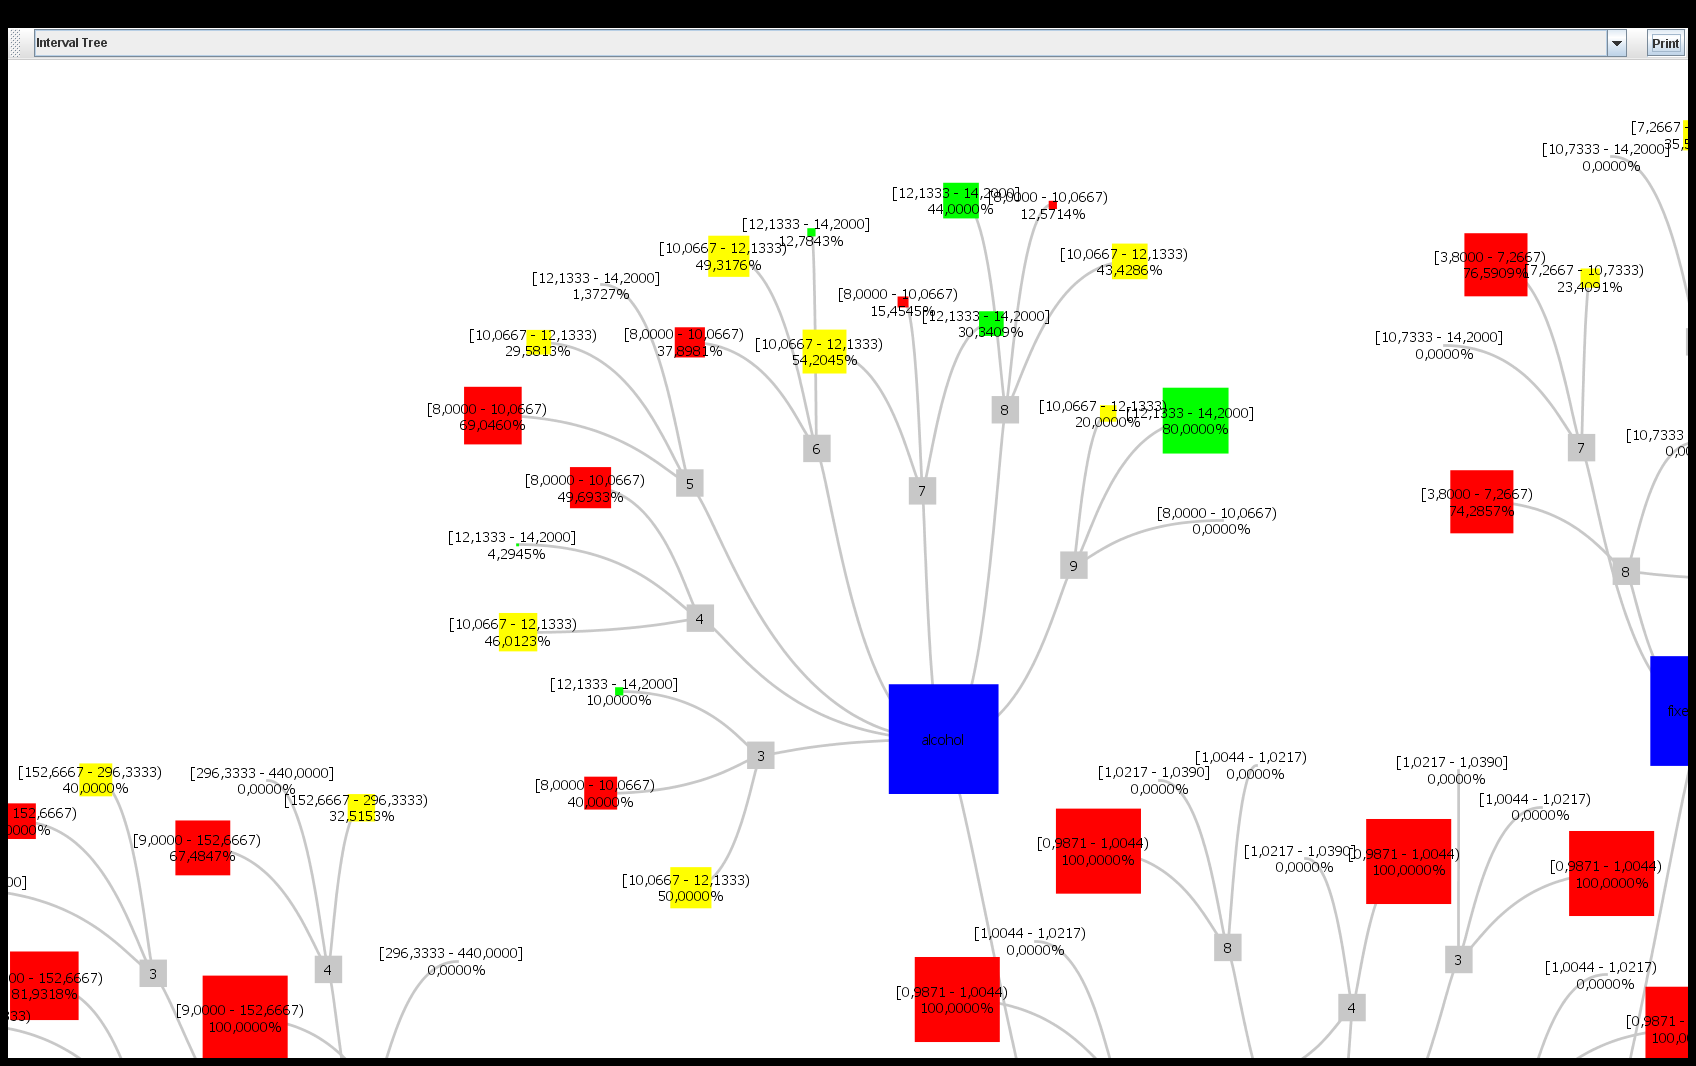
\includegraphics[width=\textwidth]{20131105034138plot.png}
  \caption{The alcohol branche in more detail}
  \label{ait}
\end{figure}

As I mentioned before this type of graph did not always gives a nice result. A good example can be found when we look at the density branch shown in figure \ref{rsit}. Even when we increased the number of intervals to 5 we still only get big red squares and not a lot of variation. This is clearly useless to analyse.
\begin{figure}[!h]
  \centering
  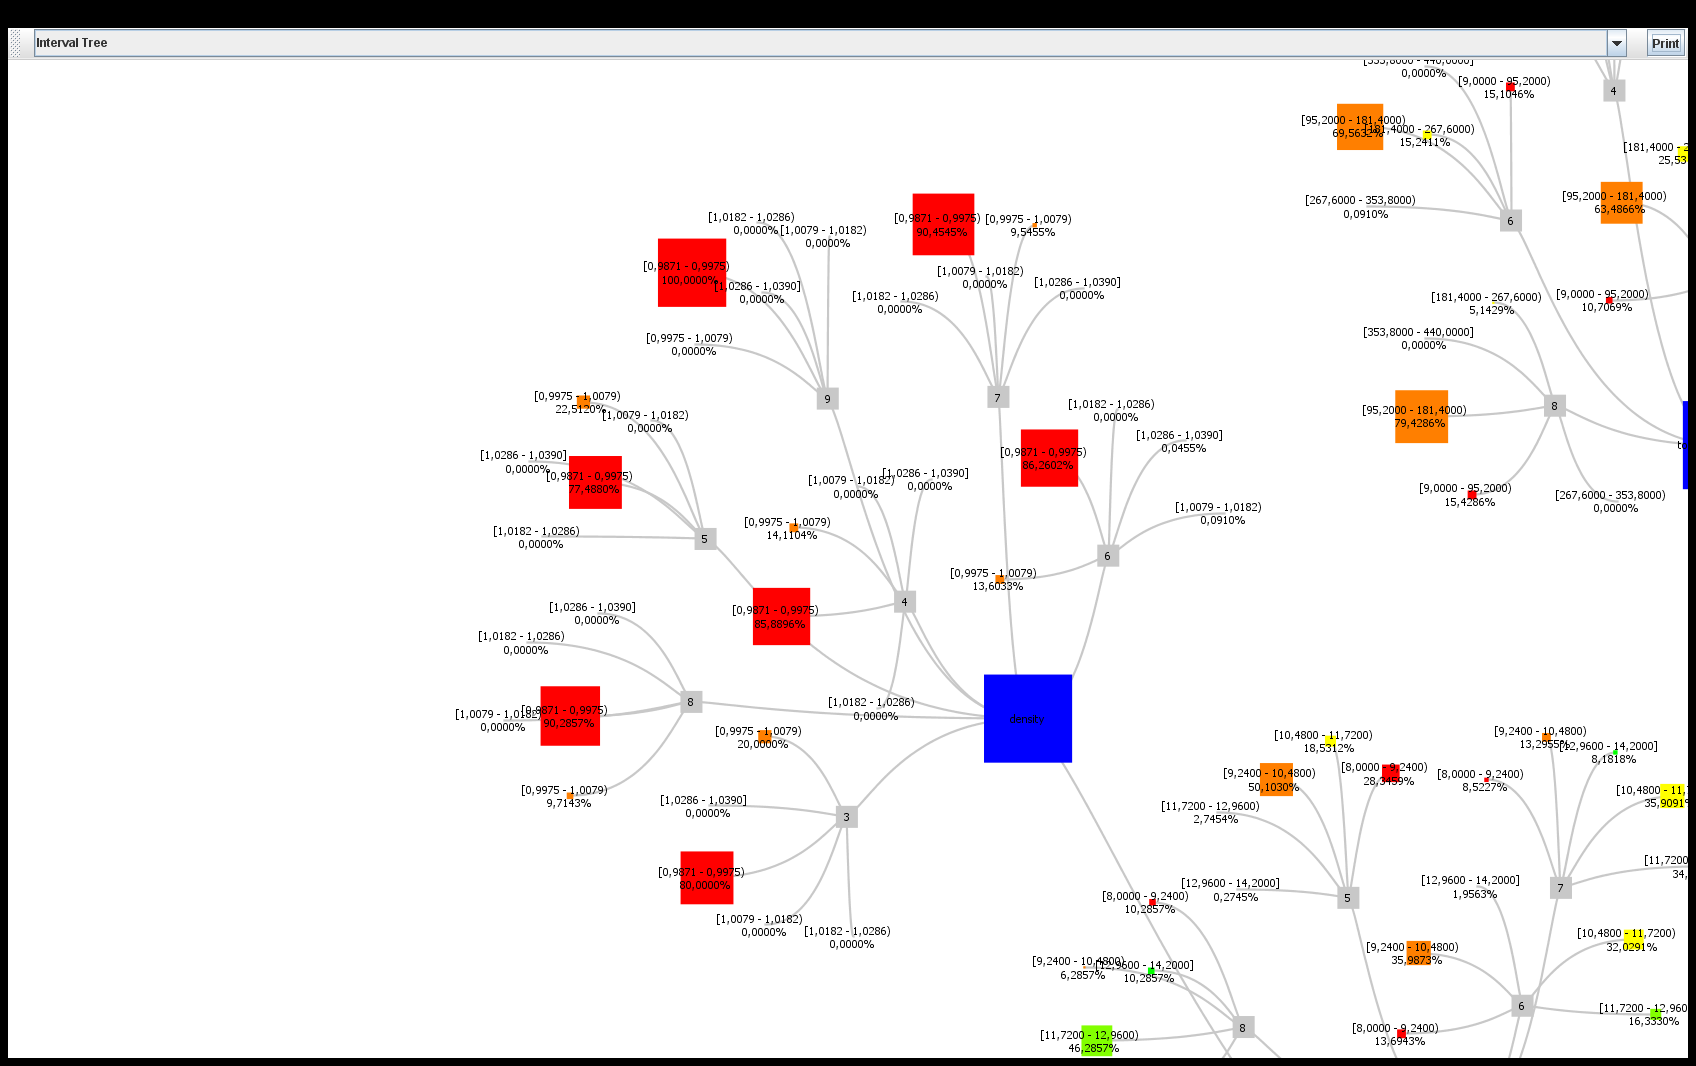
\includegraphics[width=\textwidth]{20131105041005plot.png}
  \caption{The density branch in more detail in the Interval Tree}
  \label{rsit}
\end{figure}

Now lets use the Median tree. as can be seen in figure \ref{rsmt} The result is better, we now can definitely see that lower density is better.
\begin{figure}[!h]
  \centering
  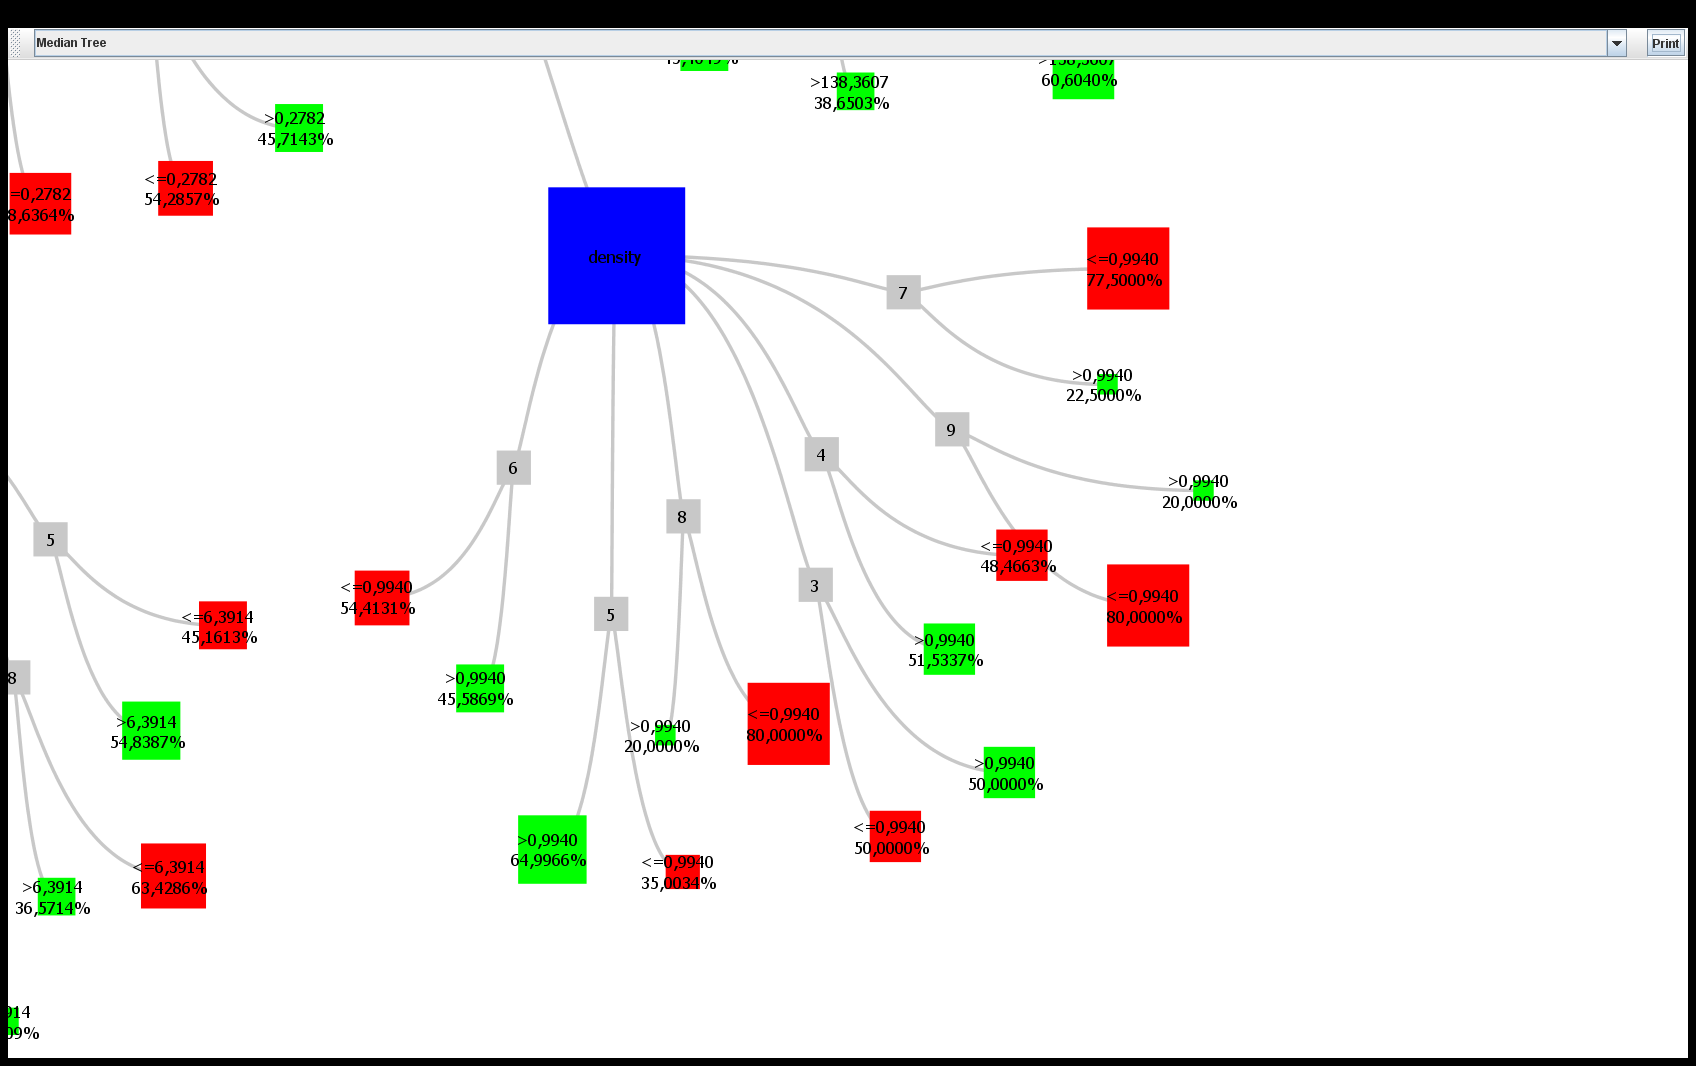
\includegraphics[width=\textwidth]{20131105041127plot.png}
  \caption{The density branch in more detail in the Median Tree}
  \label{rsmt}
\end{figure}

\section{Conclusions}
So after looking around in the Median Tree we can see that to get a top wine we need to have a high alcohol and sulfur dioxide rate but low density, chlorides, total and residual sugar sulfur dioxide.

\end{document}
